\documentclass[10pt,openright,twoside,french]{book}

\input philippe2013
\input philippe2013_cours
\input philippe2013_sections
\input philippe2013_chapitre

\usepackage{docmute}

\begin{document}
\renewcommand\MaCouleur{Purple}

%___________________________
%===    Page de garde
%------------------------------------------------------

\frontmatter

\titlepage{
\begin{center}
{\Large\bfseries\color{\MaCouleur} Philippe \bsc{De Sousa}}

\vspace*{\stretch{1}}


\begin{tikzpicture}
\begin{scope}[scale=2.5,cap=round,xshift=-3cm,yshift=1.5cm]
    % Local definitions
    \def\costhirty{0.8660256}
    % Colors
    \colorlet{anglecolor}{green!50!black}
    \colorlet{sincolor}{red}
    \colorlet{tancolor}{orange!80!black}
    \colorlet{coscolor}{blue}
    % Styles
    \tikzstyle{axes}=[]
    \tikzstyle{important line}=[very thick]
    \tikzstyle{information text}=
    [rounded corners,fill=red!10,inner sep=1ex]
    % The graphic
    \draw[style=help lines,step=0.5cm] (-1.4,-1.4) grid (1.4,1.4);
    \draw (0,0) circle (1cm);
    \begin{scope}[style=axes]
        \draw[->] (-1.5,0) -- (1.5,0) node[right] {$x$} coordinate(x axis);
        \draw[->] (0,-1.5) -- (0,1.5) node[above] {$y$} coordinate(y axis);
        \foreach \x/\xtext in {-1, -.5/-\frac{1}{2}, 1} \draw[xshift=\x cm] (0pt,1pt) -- (0pt,-1pt) node[below,fill=white] {$\xtext$};
        \foreach \y/\ytext in {-1, -.5/-\frac{1}{2}, .5/\frac{1}{2}, 1} \draw[yshift=\y cm] (1pt,0pt) -- (-1pt,0pt) node[left,fill=white] {$\ytext$};
    \end{scope}
    \filldraw[fill=green!20,draw=anglecolor] (0,0) -- (3mm,0pt) arc(0:30:3mm);
    \draw (15:2mm) node[anglecolor] {$\alpha$};
    \draw[style=important line,sincolor] (0,0) -- node[left,fill=white] {\footnotesize$\sin \alpha$} (0,0.5);
    \draw[style=important line,coscolor] (30:1cm |- x axis) -- node[below=1pt,fill=white] {\footnotesize$\cos \alpha$} (0,0);
    \draw[dashed] (30:1cm |- x axis) -- (30:1cm) -- (30:1cm -| y axis);
    \draw[style=important line,tancolor] (1,0) -- node[right,fill=white] {\footnotesize\rotatebox{-90}{$\tan \alpha$}} (intersection of 0,0--30:1cm and 1,0--1,1) coordinate (t);
    \draw (0,0) -- (t);
\end{scope}

\begin{scope}[scale=1.5,yshift=-5cm,xshift=-3cm]
%\draw[black,fill=gray!20](.445,0)node[below] {$\alpha$}--++(0,.434)node[above] {$f(\alpha)$}--plot[domain=.445:2/pi](\x,{\x*abs(sin(2/(rad(\x))))})--cycle;
\draw[blue,thick,domain=-0.5:3.2,samples=200]plot(\x,{exp(\x-2)}) node[right]{$\calig C$};
\draw[red,thick,domain=1.2:3.2,samples=200]plot(\x,{\x-1}) node[right]{$T$};
\draw[gray] (2,1) node {$\bullet$};
\draw[dashed,very thin, gray] (2,-0.5) node[below] {\tiny $x_0$} |- (2,1) -| +(1,1);
\draw[color=orange] (3,1) -- +(0,1) node[midway,fill=white,right] {\tiny\rotatebox{-90}{$f'(x_0)$}};
\draw[color=gray] (2.5,1) node[fill=white] {\tiny 1};
\draw[thick,->](-0.5,-0.5)--(4,-0.5)node[below]{$x$};%axe x
\draw[thick,->](1,-1)--(1,{exp(1.25)})node[left]{$y$};%axe y
\end{scope}

\begin{scope}[scale=1.75,>=latex,yshift=6cm,xshift=0.5cm]
    \coordinate (O) at (0,0); \draw[fill=black] (O) circle (1.5pt);
    \draw (0,0) -- ++(50:2cm);
    \coordinate (A) at (1.5,1.32); \draw[ball color=blue!25] (A) circle (0.3cm);
    \draw (1.8,1.32) -- ++ (0,-1.52cm);
    \draw[shade] (1.5,-0.2) rectangle ++(0.6,-0.2);
    \draw (0,0) -- ++(150:1.75cm);
    \coordinate (B) at (-1.67,0.62); \draw[ball color=blue!25] (B) circle (0.3cm);
    \draw (-1.97,0.62) -- ++ (0,-2.32cm);
    \draw[shade] (-2.27,-1.7) rectangle ++(0.6,-0.4);
    \draw (O) -- ++(0,-1.5cm);
    \draw[shade] (-0.3,-1.5) rectangle ++(0.6,-0.25);
    \draw (0,-0.25) arc (-90:50:0.25cm);
    \draw[double] (50:0.25cm) arc (50:150:0.25cm);
    \draw[dashed] (150:0.25cm) arc (150:270:0.25cm);
    \begin{tiny}
        \draw[->,thick,red](50:1.5pt) -- ++(50:0.75cm) node[midway,right] {$\vect u$};
        \draw[->,thick,green](150:1.5pt) -- ++(150:0.75cm) node[near end,below] {$\vect v$};
        \draw[->,thick,blue](-90:1.5pt) -- ++(-90:0.75cm) node[near end,right] {$\vect w$};
        \draw (-20:0.32cm) node {$\gamma$};
        \draw (90:0.32cm) node {$\alpha$};
        \draw (210:0.32cm) node {$\beta$};
    \end{tiny}
\end{scope}
\end{tikzpicture}
\vspace*{\stretch{1}}

\begin{tikzpicture}[remember picture,overlay]
\begin{scope}
\node [rotate=45,scale=10,text opacity=0.2]
at (current page.center) {\color{\MaCouleur} Mathématiques};
\end{scope}

\begin{scope}[xshift=5cm,yshift=10.5cm,overlay]
\draw[\MaCouleur] (0,0) node[scale=8] {\premiere};
\draw[\MaCouleur] (-0.2,-0.15) node[below,scale=6] {\sti};
\end{scope}
\end{tikzpicture}


D'après le programme $\NP{2012}$
\end{center}
} 

\pieddepage{}{}{}
\entete{}{}{}

\tableofcontents

\mainmatter

\entete{}{\color{\MaCouleur} \textbullet~\leftmark~\textbullet}{}
\pieddepage{}{%
\begin{tikzpicture}[scale=0.65]
\shadedraw [top color=white, bottom color=\MaCouleur, draw=\MaCouleur]
[l-system={Sierpinski triangle, step=1pt, angle=60, axiom=F, order=6.5}]
lindenmayer system -- cycle;
\draw (30:0.65cm) node {\bfseries\textcolor{black}{\thepage}};
\end{tikzpicture}%
}{}
%\pieddepage{}{\color{\MaCouleur}$\stackrel{***}{\thepage}$}{}

%------ Chapitre 01
    \renewcommand\PartProgramme{Stats/Probas}
    \documentclass[10pt,openright,twoside,french]{book}

\input philippe2013
\input philippe2013_cours
\input philippe2013_sections
\input philippe2013_chapitre
\renewcommand\PartProgramme{Stats/Probas}
\renewcommand\MaCouleur{Purple}

\pieddepage{}{%
\begin{tikzpicture}[scale=0.65]
\shadedraw [top color=white, bottom color=\MaCouleur, draw=\MaCouleur]
[l-system={Sierpinski triangle, step=1pt, angle=60, axiom=F, order=6.5}]
lindenmayer system -- cycle;
\draw (30:0.65cm) node {\bfseries\textcolor{black}{\thepage}};
\end{tikzpicture}%
}{}


\begin{document}
\chapter{Statistiques descriptives}\label{ch_stats}

\section{Vocabulaire}

Une \textbf{étude statistique} a pour but d'obtenir une information, appelée \textbf{caractère}, sur une population à partir de \textbf{données} recueillies sur un \textbf{échantillon} de cette population.

\begin{Defi}
    Le \iptb{caractère}\index{caractère!les différents types de} étudié peut être :
    \begin{description}
        \item[quantitatif :] les valeurs du caractère s'expriment avec des nombres (ex : températures, pointures, salaires\ldots) ;
        \item[qualitatif :] les valeurs ne s'expriment pas par des nombres (ex : couleurs, type d'essence\ldots) ;
        \item[discret :] les valeurs du caractère sont isolés (ex : notes\ldots) ;
        \item[continu :] les valeurs sont regroupées par classes (ou intervalles de nombre) (par ex : durée, distance parcourue,
    \end{description}
\end{Defi}

\begin{Rmq}
    Dans la suite du cours, on considère que le caractère est quantitatif.
\end{Rmq}

\begin{Defi}
    Lorsque les valeurs d'une série statistique sont regroupés par classe de type $\intervallefo a b$, on appelle \ipt{centre de classe} le nombre défini par $\frac{a + b}{2}$.
\end{Defi}

\section{Indicateurs de position}
\subsection{Moyenne}
\begin{Defi}
On considère une série qui possède des valeurs différentes $x_1, x_2, \ldots, x_p$ chacune affectée de leur effectif. L'effectif total est égal à $N$.\par
On appelle \ipt{moyenne} d'une série le nombre $\overline{m}$ tel que :
\[\overline{m} = \frac{n_1x_1 + n_2x_2 + n_3x_3 + \cdots + n_px_p}{n_1 + n_2 + \cdots + n_p} = \frac{\displaystyle\sum_{i =1}^{p}n_ix_i}{N}.\]
\end{Defi}

\begin{Exemple}
    Un élève souhaite calculer la moyennes de ses notes sur $20$ : $8 \pv 10 \pv 14 \pv 13 \pv 10 \pv 14 \pv 10$.\par\medskip
    $\overline m = \frac{8 + 10 + 14 + 13 + 10 + 14 + 10}{7} = \frac{79}{7} \approx 11,29$.\medskip

    Parfois, les valeurs sont regroupées dans un tableau : \quad
    \begin{tabular}{*{5}{|c}|}
    \hline
        Notes & $8$ & $10$ & $13$ & $14$ \\
    \hline
        Effectifs & $1$ & $3$ & $1$ & $2$ \\
    \hline
    \end{tabular}\par\medskip
    On peut alors utiliser la formule : $\overline m = \frac{1 \times 8 + 3 \times 10 + 1 \times 13 + 2 \times 14}{1 + 3 + 1 + 2} = \frac{79}{7} \approx 11,29.$
\end{Exemple}

\begin{Rmq}[s]
\begin{enumerate}
    \item En règle générale, la moyenne n'est pas une valeur de la série. On peut la considérer comme le \textnormal{point d'équilibre} des valeurs. Par conséquent, la moyenne est sensible aux valeurs extrêmes.\par
        Pour reprendre l'exemple, si la prochaine note du contrôle est très élevée alors la moyenne va augmenter.
    \item Lorsque les valeurs sont regroupés par classe, au lieu d'utiliser les $x_i$, on utilise les centres de classe.
\end{enumerate}
\end{Rmq}

\begin{Exemple}
    Le tableau ci-dessous regroupe le temps de parcours des habitants d'un village entre leur domicile et leur lieu de travail. Le maire cherche à calculer le temps moyen.
    \begin{center}
    \renewcommand\arraystretch{1.5}
        \begin{tabular}{*{7}{|c}|}
            \hline
                Durée en min & $[0 \pv 10[$ & $[10 \pv 20[$ & $[20 \pv 30[$ & $[30 \pv 50[$ & $[50 \pv 70[$ & Total \\
            \hline
                Effectif & $18$ & $35$ & $25$ & $112$ & $80$ & $270$ \\
            \hline
                Centre de classe & $5$ & $15$ & $25$ & $40$ & $60$ & \\
            \hline
        \end{tabular}
    \renewcommand\arraystretch{1}
    \end{center}
    On a donc : $\overline m = \frac{18 \times 5 + 35 \times 15 + 25 \times 25 + 112 \times 40 + 80 \times 60}{270} = \frac{\NP{10520}}{270} \approx 39~min.$
\end{Exemple}

\subsection{Médiane}

\begin{Defi}
    On considère une série statistique dont l'effectif total est égal à $N$. Les valeurs sont rangées dans l'ordre croissant.

    \textbf{Une} \ipt{médiane} $Me$ est un nombre réel qui permet de partager la série statistique en deux séries de même valeur.

    Autrement dit, la moitié ($50\%$) des valeurs de la série est inférieure ou égale à $Me$ et l'autre moitié est supérieure ou égale à $Me$.

\begin{center}
    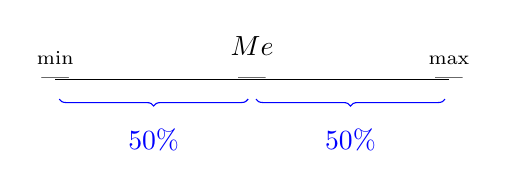
\begin{tikzpicture}
        \draw (0,0)--(5,0) node[midway] {|} node[midway,above=5pt] {$Me$};
        \draw (0,0) node {|} node[above=2pt] {\scriptsize $\min$}; \draw (5,0) node {|} node[above=2pt] {\scriptsize $\max$};
        \draw[color=blue,decorate,decoration={brace,raise=0.25cm}] (2.45,0) -- (0.05,0) node[below=0.5cm,pos=0.5] {$50\%$};
        \draw[color=blue,decorate,decoration={brace,raise=0.25cm}] (4.95,0) -- (2.55,0) node[below=0.5cm,pos=0.5] {$50\%$};
    \end{tikzpicture}
\end{center}
\end{Defi}

\textbf{Méthode de calcul :} Par définition, la médiane dépend de l'effectif de la série :
\begin{itemize}
    \item Si $N$ est impair, alors on calcule $\frac{N + 1}{2}$ et le résultat correspond à la position de la médiane choisie dans la série.
    \item Si $N$ est pair, alors la médiane choisie est égale à la moyenne de la valeur situé à la position $\frac N 2$ et la valeur suivante.
\end{itemize}

\begin{Exemple}
On considère le relevé des températures en janvier et en février dans une ville :
\begin{center}
\renewcommand\arraystretch{1.5}
    \begin{tabular}{*{10}{|c}|}
        \hline
            \multicolumn{10}{|c|}{Janvier}\\
        \hline
            Valeurs & $-3\degres$ & $-2\degres$ & $-1\degres$ & $0\degres$ & $1\degres$ & $2\degres$ & $3\degres$ & $4\degres$ & Total \\
        \hline
            Effectifs & $3$ & $5$ & $8$ & $5$ & $4$ & $3$ & $2$ & $1$ & $31$\\
        \hline
            \multicolumn{10}{|c|}{Février}\\
        \hline
            Valeurs & $-3\degres$ & $-2\degres$ & $-1\degres$ & $0\degres$ & $1\degres$ & $2\degres$ & $3\degres$ & $4\degres$ & Total \\
        \hline
            Effectifs & $1$ & $2$ & $3$ & $3$ & $5$ & $9$ & $3$ & $2$ & $28$\\
            \hline
    \end{tabular}
\renewcommand\arraystretch{1}
\end{center}\medskip

\begin{description}
    \item[En janvier :] $N = 31$ donc $\frac{N+1}{2} = 16$ : une médiane possible est la $16$\ieme valeur donc $Me = -1\degres$. En janvier, il a fait moins de $-1\degres$ la moitié du mois.
    \item[En févier :] $N = 28$ donc $\frac{N}{2} = 14$ : la $14\ieme$ est $1\degres$ et la suivante est égale à $2\degres$. Donc la moyenne des deux est $\frac{1+2}{2} = 1,5$. Une médiane possible est égale à $1,5\degres$ donc durant la moitié du mois, la température a été supérieure à $1,5\degres$.
\end{description}
\end{Exemple}

\begin{Rmq}
    Contrairement à la moyenne, la médiane n'est pas sensible aux valeurs extrêmes. En effet, dans notre exemple, si la dernière température était égale à $20\degres$ au lieu de $4\degres$, la moyenne augmenterait alors que la médiane resterait identique car l'effectif total n'a pas changé.
\end{Rmq}

\subsection{Quartiles}

\begin{Defi}
    On considère une série statistique $S$ dont l'effectif total est égal à $N$. Les valeurs sont rangées dans l'ordre croissant.
    \begin{itemize}
        \item Le \ipt{premier quartile}\index{quartile} $Q_1$ de $S$ est le plus petit élément $a$ de $S$ tel qu'au moins $25\%$ des données soient inférieures ou égales à $a$.
        \item Le \ipt{troisième quartile}\index{quartile} $Q_3$ de $S$ est le plus petit élément $b$ de $S$ tel qu'au moins $75\%$ des données soient inférieures ou égales à $b$.
    \end{itemize}

\begin{center}
    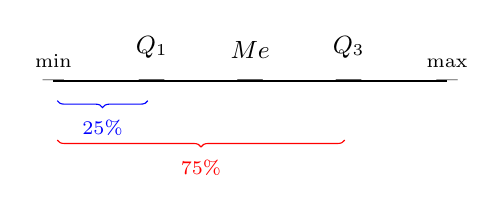
\begin{tikzpicture}
        \begin{small}
        \draw (0,0)--(5,0) node[midway] {|} node[midway,above=5pt] {$Me$} node[pos=0.75,above=5pt] {$Q_3$} node[pos=0.25,above=5pt] {$Q_1$};
        \draw (0,0)--(5,0) node[pos=0.25] {|}; \draw (0,0)--(5,0) node[pos=0.75] {|};
        \end{small}
        \begin{scriptsize}
        \draw (0,0) node {|} node[above=2pt] {$\min$}; \draw (5,0) node {|} node[above=2pt] {$\max$};
        \draw[color=blue,decorate,decoration={brace,raise=0.25cm}] (1.2,0) -- (0.05,0) node[below=0.4cm,pos=0.5] {$25\%$};
        \draw[color=red,decorate,decoration={brace,raise=0.75cm}] (3.7,0) -- (0.05,0) node[below=0.9cm,pos=0.5] {$75\%$};
        \end{scriptsize}
    \end{tikzpicture}
\end{center}
\end{Defi}

\textbf{Méthode de calcul :} Par définition, les quartiles dépendent de l'effectif de la série :
\begin{description}
    \item[Premier quartile :] On arrondit le nombre $\frac{N}{4}$ à l'unité par excès et cela donne la position de $Q_1$ dans la série $S$.
    \item[Troisième quartile :] On arrondit le nombre $3\times\frac{N}{4}$ à l'unité par excès et cela donne la position de $Q_3$ dans la série $S$.
\end{description}

\begin{Exemple}
    On reprend les températures du moins de janvier de l'exemple précédent.
    \begin{description}
        \item[Premier quartile :] $N = 31$ donc $\frac N 4 = 7,75 \approx 8$ donc la $8\ieme$ valeur est $Q_1 = -2\degres$.
        \item[Troisième quartile :] $N = 31$ donc $3\times\frac N 4 = 23,25 \approx 24$ donc la $24\ieme$ valeur donne $Q_3 = 1\degres$.
    \end{description}
    Ainsi, $25\%$ des valeurs sont inférieures ou égales à $-2\degres$ et $75\%$ des valeurs sont inférieures ou égales à $1\degres$. On peut dire aussi que $25\%$ des valeurs sont supérieures ou égales à $1\degres$.
\end{Exemple}

\section{Indicateurs de dispersion}

Dans les classes antérieures, l'\iptb{étendue} était un indicateur de dispersion utilisé dont voici rappelée la définition :

\begin{Defi}
    Dans une série statistique, l'\iptb{étendue}\index{etendue@étendue} est la différence entre la valeur maximale et la valeur minimale.
\end{Defi}

\begin{Rmq}
    Une valeur élevée de l'étendue signifie qu'au moins une des valeurs extrêmes de la série est éloignée de la médiane et le risque de dispersion des valeurs est donc plus important.\par
    Dans l'exemple précédent, l'étendue de la série \textnormal{janvier} était identique à celle de la série \textnormal{février} ce qui montre les besoins d'avoir d'autres indicateurs.\par
    Les quartiles nous permettent d'obtenir d'autres indicateurs de dispersion lié à la médiane.
\end{Rmq}

\subsection{Intervalle et écart interquartile}

\begin{Defi}
    On appelle l'\ipt{intervalle interquartile} l'intervalle $\intervalleff{Q_1}{Q_3}$.\par
    On appelle l'\iptb{écart interquartile}\index{ecart interquartile@écart interquartile} le nombre $Q_3 - Q_1$.
\end{Defi}

\begin{Rmq}
\begin{center}
    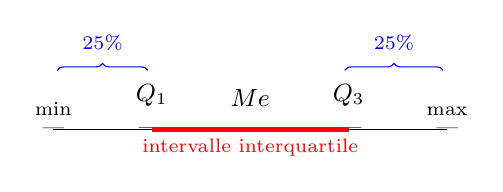
\begin{tikzpicture}
        \begin{small}
        \draw (0,0)--(5,0) node[midway] {|} node[midway,above=5pt] {$Me$} node[pos=0.75,above=5pt] {$Q_3$} node[pos=0.25,above=5pt] {$Q_1$};
        \draw (0,0)--(5,0) node[pos=0.25] {|}; \draw (0,0)--(5,0) node[pos=0.75] {|};
        \end{small}
        \begin{scriptsize}
        \draw (0,0) node {|} node[above=2pt] {$\min$}; \draw (5,0) node {|} node[above=2pt] {$\max$};
        \draw[color=blue,decorate,decoration={brace,raise=0.75cm}] (0.05,0) -- (1.2,0) node[above=0.9cm,pos=0.5] {$25\%$};
        \draw[color=blue,decorate,decoration={brace,raise=0.75cm}] (3.7,0) -- (4.95,0) node[above=0.9cm,pos=0.5] {$25\%$};
        \draw[red,line width=2pt] (1.25,0)--(3.75,0) node[midway,below] {intervalle interquartile};
        \end{scriptsize}
    \end{tikzpicture}
\end{center}

La figure ci-dessus nous permet de comprendre pourquoi l'intervalle interquartile contient $50\%$ de valeurs de la série, c'est-à-dire la moitié. Ainsi, un écart interquartile faible impose que les valeurs soient regroupées proches de la médiane et donc peu dispersée pour la moitié d'entre elles.
\end{Rmq}

\subsection{Variance et écart-type}
On s'intéresse ici à l'écart existant entre chaque valeur de la série et la moyenne. Puis on calcule la moyenne de ces écarts. Dans ce cas, on trouve $0$. En effet :
\[\begin{split}
    \frac{x_1 - \overline m + x_2 - \overline m + \cdots + x_n - \overline m}{n} &= \frac{x_1 + x_2 + \cdots x_n}{n} - \frac{n \times \overline m}{n} \\
    &= \overline m - \overline m \\
    &= 0
\end{split}\]

Pour éviter ce résultat, on utilise la même méthode mais en calculant la moyenne des carrés des écarts.

\begin{Defi}
    Soit $S$ une série statistique de valeurs $x_1$, $x_2, \ldots, x_n$ et de moyenne $\overline m$. La \ipt{variance} est le nombre positif ou nul $V$ défini par :
    \[V = \frac{(x_1 - \overline m)^2 + (x_2 - \overline m)^2 + \cdots + (x_3 - \overline m)^2}{n} = \frac1n \sum_{i = 1}^{n}(x_i - \overline m)^2.\]
\end{Defi}

\begin{Exemple}
    Prenons une série de notes :
    \begin{center}
    \renewcommand\arraystretch{2}
        \begin{tabular}{|c|*{6}{m{1.5cm}|}}
            \hline
                Notes & $7$ & $9$ & $12$ & $13$ & $15$ & $18$ \\
            \hline
                Effectifs & $1$ & $2$ & $1$ & $2$ & $4$ & $2$ \\
            \hline
                \multicolumn{7}{|c|}{Moyenne : $\overline m = 159 \div 12 = 13,25$} \\
            \hline
                $(x_i - \overline m)$ & $-6,25$ & $-4,25$ & $-1,25$ & $-0,25$ & $1,75$ & $4,75$ \\
            \hline
                $(x_i - \overline m)^2$  & $39,0625$  & $18,0625$ & $1,5625$ &$0,0625$ & $3,0625$ & $22,5625$  \\
            \hline
                \multicolumn{7}{|c|}{Variance : $V = (39,0625 \times 1 + 18,0625 \times 2 + \cdots + 22,5625 \times 2) \div 12 = 134,25 \div 12 = 11,1875$} \\
            \hline
        \end{tabular}
    \renewcommand\arraystretch{1}
    \end{center}
    La moyenne des carrés des écarts est donc égale à $11,1875$.
\end{Exemple}

\begin{Thm}[de König-Huygens (admis)]
    Soit $S$ une série statistique de valeurs $x_1$, $x_2, \ldots, x_n$ et de moyenne $\overline m$.\par
    On pose $\overline n = \frac{x_1^2 + x_2^2 + \cdots + x_n^2}{n}$ (moyenne des carrés des valeurs).\par
    La variance $V$ de la série statistique est alors égale à :
    \[V = \overline n - (\overline m)^2.\]
\end{Thm}\clearpage

\begin{Exemple}
    Avec l'exemple précédent :
    \begin{center}
    \renewcommand\arraystretch{2}
        \begin{tabular}{|c|*{6}{m{1.5cm}|}}
            \hline
                Notes & $7$ & $9$ & $12$ & $13$ & $15$ & $18$ \\
            \hline
                Effectifs & $1$ & $2$ & $1$ & $2$ & $4$ & $2$ \\
            \hline
                \multicolumn{7}{|c|}{Moyenne : $\overline m = 159 \div 12 = 13,25$} \\
                \multicolumn{7}{|c|}{donc $(\overline m)^2 = 175,5625$} \\
            \hline
                $(x_i)^2$ & $49$ & $81$ & $144$ & $169$ & $225$ & $324$ \\
            \hline
                \multicolumn{7}{|c|}{Moyenne des carrés : $\overline n = \NP{2241} \div 12 = 186,75$} \\
            \hline
                \multicolumn{7}{|c|}{Variance : $V = 186,75 - 175,5625 = 11,1875$} \\
            \hline
        \end{tabular}
    \renewcommand\arraystretch{1}
    \end{center}
    On trouve bien le même résultat mais en faisant intervenir la moyenne qu'une seule fois.
\end{Exemple}\medskip

Cela n'est cependant pas exploitable car l'unité de mesure n'est plus la même depuis que l'on a utilisé des nombres au carré. On s'intéresse donc surtout à l'indicateur suivant :\medskip

\begin{Defi}
    Soit $S$ une série statistique de variance $V$. L'\iptb{écart-type}\index{ecart-type@écart-type} $\sigma$ est le nombre réel positif défini par : \[\sigma = \sqrt V.\]
\end{Defi}

\begin{Rmq}
    L'écart-type est un nombre réel positif qui caractérise la dispersion des valeurs d'une série statistiques par rapport à la moyenne.\par
    Plus l'écart-type est petit et plus les valeurs sont proches de la moyenne (dispersion faible). Au contraire, si l'écart-type est grand alors les valeurs sont éloignés de la moyenne (dispersion élevée).\par
    Calculer l'écart-type est notamment intéressant pour comparer plusieurs séries statistiques dont les valeurs sont exprimées dans la même unité de mesure.
\end{Rmq}\medskip

\begin{Exemple}
    Dans l'exemple précédent, on obtient $\sigma = \sqrt{11,1875} \approx 3,34$.\par
    Cela donne une indication de la répartition moyenne des notes autour de la moyenne $\overline m$.
\end{Exemple}

\begin{Rmq}
    En \premiere\sti, on utilisera la plupart du temps la calculatrice ou le tableur pour calculer directement la variance et l'écart-type.\par
    On se servira alors des fonctions \bsc{\texttt{var.p}} et \bsc{\texttt{ecartypep}} ou encore, pour la dernière version de \bsc{\texttt{Excel}} : \bsc{\texttt{var.p.n}} et \bsc{\texttt{ecartype.pearson}}
\end{Rmq}



\end{document}


%------ Chapitre 02
    \renewcommand\PartProgramme{Analyse}
    \documentclass[10pt,openright,twoside,french]{book}

\input philippe2013
\input philippe2013_cours
\input philippe2013_sections
\input philippe2013_chapitre
\renewcommand\PartProgramme{Analyse}
\renewcommand\MaCouleur{Purple}

%\pieddepage{}{%
%\begin{tikzpicture}[scale=0.65]
%\shadedraw [top color=white, bottom color=\MaCouleur, draw=\MaCouleur]
%[l-system={Sierpinski triangle, step=1pt, angle=60, axiom=F, order=6.5}]
%lindenmayer system -- cycle;
%\draw (30:0.65cm) node {\bfseries\textcolor{black}{\thepage}};
%\end{tikzpicture}%
%}{}

\setcounter{chapter}{1}
\begin{document}
\chapter{\'Etudes de fonctions}\label{ch_etudes_fonctions}

\section{Fonction $x \mapsto  \abs x$}

\begin{Defi}
    Pour tout $x \in \R$, on définit la fonction \ipt{valeur absolue} $x \mapsto \abs x$ par :
    \[\abs{x} =
    \left\{\begin{array}{r@{\quad\text{si}\quad}l}
         x & x \geq 0 \\
        -x & x < 0
    \end{array}\right.\]
\end{Defi}

La définition nous permet de déduire immédiatement le résultat suivant :

\begin{Prop}
    Pour tout $x \in \R^*$, la fonction valeur absolue est strictement positive et $\abs 0 = 0$.\par
    Son minimum (la plus petite des images) est donc égal à $0$.
\end{Prop}

D'après la définition, on constate que la fonction valeur absolue est une fonction affine par morceaux.\par
En effet, pour $x < 0$, elle est égale à la fonction affine $x \mapsto -x$ et elle est donc décroissante.\par
Pour $x \geq 0$, elle est égale à la fonction affine $x \mapsto x$ et elle est donc croissante.\par
On en déduit alors sa représentation graphique ainsi que ses variations.

\begin{center}
    \begin{tikzpicture}[>=latex]
        \draw[->] (-5,0) -- (5,0) node[below] {$x$} ;
        \foreach \x in {-4, -3,...,-1} \draw[xshift=\x cm] (0pt,2pt) -- (0pt,-2pt) node[below] {$\x$};
        \foreach \x in {1, 2,...,4} \draw[xshift=\x cm] (0pt,2pt) -- (0pt,-2pt) node[below] {$\x$};
        \draw[->] (0,-1) -- (0,5) node[left] {$y$} ;
        \foreach \y in {1,2,...,4} \draw[yshift=\y cm] (-2pt,0pt) -- (2pt,0pt) node[left=1.5pt] {$\y$};
        \draw (0,0) node[below left] {$0$};
        \draw[blue,thick,domain=-4.75:4.75,samples=200]plot(\x,{abs(\x)}) node[right]{$\abs x$};
        \draw (-2.5,2.5) node[above=-3mm] {\rotatebox{-45}{$\abs x = -x$}};
        \draw (2.5,2.5) node[above=-3mm] {\rotatebox{45}{$\abs x = x$}};
    \end{tikzpicture}
\end{center}

\begin{Prop}
    Sur l'intervalle $\intervalleof{-\infty}{0}$, la fonction valeur absolue est strictement décroissante.\par
    Sur l'intervalle $\intervallefo{0}{+\infty}$, la fonction valeur absolue est strictement croissante.
\end{Prop}

\begin{center}
    \begin{tikzpicture}
        \tkzTabInit[color,espcl=4]%
        {$x$ /1, Variations\\ de $\abs x$ /1.5}%
        {$-\infty$,$0$,$+\infty$}%
        \tkzTabVar[color=red]{ +/ ,-/ $0$,+ /}
    \end{tikzpicture}
\end{center}

\begin{Rmq}
    La fonction valeur absolue étant toujours positive ou nulle, sa représentation graphique est au-dessus de l'axe des abscisses.
\end{Rmq}\medskip

En enfin, toujours grâce aux fonctions affines, on a le résultat graphique suivant :

\begin{Prop}
    La représentation graphique de la fonction valeur absolue est symétrique par rapport à l'axe des ordonnées.
\end{Prop}

\section{Somme et fonctions composées}
On se place dans un repère orthonormé nommé $(O, I, J)$. On considère une fonction $u$ définie sur $\calig D_u$ dont voici la représentation graphique $\calig C_u$ sur un intervalle $A$.

\begin{center}
    \begin{tikzpicture}
        \draw[->] (-1.75,0)--(4,0) node[below] {$x$};
        \draw[->] (0,-0.25)--(0,4) node[left] {$y$};
        \draw (0,0) node[below left] {\small $O$};
        \draw (1,0) node[below=2pt] {\small $I$} node {|};
        \draw (0,1) node[left=2pt] {\small $J$} node {--};
        \draw[color=red,line width=1pt] plot[domain=-1.25:3.6,samples=200] (\x,{cos(deg(\x+0.2))+0.5});
    \end{tikzpicture}
\end{center}

\subsection{Fonction $t \mapsto u(t) + k$}

\begin{Prop}[(admise)]
    La représentation graphique de la fonction $t \mapsto u(t) + k$ est l'image de $\calig C_u$ par la translation de vecteur $k\times\vect{OJ}$.
\end{Prop}

\begin{center}
    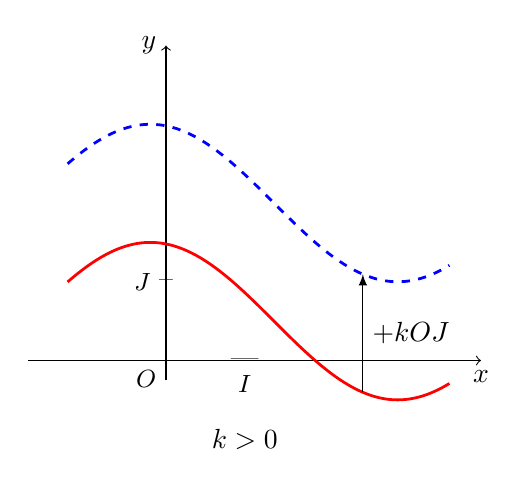
\begin{tikzpicture}
        \draw[->] (-1.75,0)--(4,0) node[below] {$x$};
        \draw[->] (0,-0.25)--(0,4) node[left] {$y$};
        \draw (0,0) node[below left] {\small $O$};
        \draw (1,0) node[below=2pt] {\small $I$} node {|};
        \draw (0,1) node[left=2pt] {\small $J$} node {--};
        \draw[color=red,line width=1pt] plot[domain=-1.25:3.6,samples=200] (\x,{cos(deg(\x+0.2))+0.5});
        \draw[color=blue,line width=1pt, dashed] plot[domain=-1.25:3.6,samples=200] (\x,{cos(deg(\x+0.2))+2});
        \draw[->,>=latex,thin] (2.5,{cos(deg(2.5+0.2))+0.5}) -- (2.5,{cos(deg(2.5+0.2))+2}) node[midway,right] {$+k\vect{OJ}$};
        \draw (1,-1) node {$k > 0$};
    \end{tikzpicture}
\hspace*{1cm}
    \begin{tikzpicture}
        \draw[->] (-1.75,0)--(4,0) node[below] {$x$};
        \draw[->] (0,-0.25)--(0,4) node[left] {$y$};
        \draw (0,0) node[below left] {\small $O$};
        \draw (1,0) node[below=2pt] {\small $I$} node {|};
        \draw (0,1) node[left=2pt] {\small $J$} node {--};
        \draw[color=red,line width=1pt] plot[domain=-1.25:3.6,samples=200] (\x,{cos(deg(\x+0.2))+0.5});
        \draw[color=blue,line width=1pt, dashed] plot[domain=-1.25:3.6,samples=200] (\x,{cos(deg(\x+0.2))+0.2});
        \draw[->,>=latex,thin] (-1.2,{cos(deg(-1.2+0.2))+0.5}) -- (-1.2,{cos(deg(-1.2+0.2))+0.2}) node[midway,left] {$+k\vect{OJ}$};
        \draw (1,-1) node {$k < 0$};
    \end{tikzpicture}
\end{center}

\begin{Prop}[(admise)]
    Les fonctions $t \mapsto u(t)$ et $t \mapsto u(t) + k$ ont le même ensemble de définition.
\end{Prop}

\subsection{Fonction $t \mapsto u(t + \lambda)$}

\begin{Prop}[(admise)]
    La représentation graphique de la fonction $t \mapsto u(t + \lambda)$ est l'image de $\calig C_u$ par la translation de vecteur $-\lambda\times\vect{OI}$.
\end{Prop}

\begin{center}
    \begin{tikzpicture}
        \draw[->] (-1.75,0)--(4,0) node[below] {$x$};
        \draw[->] (0,-0.25)--(0,4) node[left] {$y$};
        \draw (0,0) node[below left] {\small $O$};
        \draw (1,0) node[above=2pt] {\small $I$} node {|};
        \draw (0,1) node[left=2pt] {\small $J$} node {--};
        \draw[color=red,line width=1pt] plot[domain=-1.25:3.6,samples=200] (\x,{cos(deg(\x+0.2))+0.5});
        \draw[color=blue,line width=1pt, dashed] plot[domain=-2.75:2.1,samples=200] (\x,{cos(deg(\x+1.7))+0.5});
        \draw[->,>=latex,thin] (-1,{cos(deg(-1+0.2))+0.5}) -- (-2.5,{cos(deg(-1+0.2))+0.5}) node[midway,below] {$-\lambda\vect{OI}$};
        \draw (1,-1) node {$\lambda > 0$};
    \end{tikzpicture}
\hspace*{0.5cm}
    \begin{tikzpicture}
        \draw[->] (-1.75,0)--(4,0) node[above] {$x$};
        \draw[->] (0,-0.25)--(0,4) node[left] {$y$};
        \draw (0,0) node[below left] {\small $O$};
        \draw (1,0) node[above=2pt] {\small $I$} node {|};
        \draw (0,1) node[left=2pt] {\small $J$} node {--};
        \draw[color=red,line width=1pt] plot[domain=-1.25:3.6,samples=200] (\x,{cos(deg(\x+0.2))+0.5});
        \draw[color=blue,line width=1pt, dashed] plot[domain=0.65:5.5,samples=200] (\x,{cos(deg(\x-1.7))+0.5});
        \draw[->,>=latex,thin] (0.5,{cos(deg(0.5+0.2))+0.5}) -- (2.4,{cos(deg(0.5+0.2))+0.5}) node[midway,below] {$-\lambda\vect{OI}$};
        \draw (1,-1) node {$\lambda < 0$};
    \end{tikzpicture}
\end{center}

\begin{Rmq}
    L'intervalle de définition de la fonction $u$ subit également une translation. Il faut donc faire attention à cela.
\end{Rmq}

\begin{Exemple}
    La fonction inverse $f \colon x \mapsto \frac 1x$ est défini sur $\R^* = \R \setminus \{0\} = \intervalleoo{-\infty}{0} \cup \intervalleoo{0}{+\infty}$.\par
    On pose maintenant la fonction $g$ définie sur $\calig D_g$ par $g(x) = f(x + a) = \frac{1}{x + a}$ où $a$ est un nombre réel. La représentation graphique de $g$ sera l'image de la représentation graphique de la fonction $f$ par le vecteur $-a\vect{OI}$. On aura donc : $\calig D_g = \R \setminus \{-a\} = \intervalleoo{-\infty}{-a} \cup \intervalleoo{-a}{+\infty}$.

\begin{center}
\begin{tikzpicture}[scale=0.5]
\begin{scope}
    \clip (-4.5,-4.5) rectangle (4.5,4.5);
        \draw[->] (-4,0)--(4,0) node[below] {$x$};
        \draw[->] (0,-4)--(0,4) node[left] {$y$};
        \draw (0,0) node[below left] {\small $O$};
        \draw (1,0) node[above=2pt] {\small $I$} node {|};
        \draw (0,1) node[left=2pt] {\small $J$} node {--};
    \draw[smooth,samples=200,domain=-4:-0.1] plot(\x,{1/\x});
    \draw[smooth,samples=200,domain=0.1:4] plot(\x,{1/\x});
\end{scope}
\begin{scope}[xshift=10cm]
    \clip (-4.5,-4.5) rectangle (4.5,4.5);
        \draw[->] (-4,0)--(4,0) node[below] {$x$};
        \draw[->] (0,-4)--(0,4) node[left] {$y$};
        \draw (0,0) node[below left] {\small $O$};
        \draw (1,0) node[above=2pt] {\small $I$} node {|};
        \draw (0,1) node[left=2pt] {\small $J$} node {--};
    \draw[smooth,samples=200,domain=-4:1.4] plot(\x,{1/(\x-1.5)});
    \draw[smooth,samples=200,domain=1.6:4] plot(\x,{1/(\x-1.5)});
    \draw[dashed, blue] (1.5,-4.5) -- (1.5,4.5) node[below right=-2pt,midway] {\scriptsize$-a$} node[midway]{$\times$};
\end{scope}
\end{tikzpicture}
\end{center}
\end{Exemple}

\subsection{Fonction $t \mapsto \abs{u(t)}$}

\begin{Prop}[(admise)]
    Deux cas se présentent :
    \begin{enumerate}
        \item Sur la réunion de tous les intervalles où la fonction $u$ est positive, alors $\calig C_u$ est confondue avec la courbe de $\abs u$.
        \item Sinon, la courbe représentative de la fonction $\abs u$ est l'image de $\calig C_u$ par la symétrie d'axe $(OI)$.
    \end{enumerate}
\end{Prop}

\begin{center}
    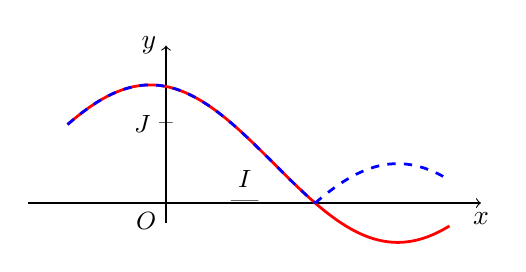
\begin{tikzpicture}
        \draw[->] (-1.75,0)--(4,0) node[below] {$x$};
        \draw[->] (0,-0.25)--(0,2) node[left] {$y$};
        \draw (0,0) node[below left] {\small $O$};
        \draw (1,0) node[above=2pt] {\small $I$} node {|};
        \draw (0,1) node[left=2pt] {\small $J$} node {--};
        \draw[color=red,line width=1pt] plot[domain=-1.25:3.6,samples=200] (\x,{cos(deg(\x+0.2))+0.5});
        \draw[color=blue,line width=1pt, dashed] plot[domain=-1.25:{rad(acos(-0.5))-0.2},samples=200] (\x,{cos(deg(\x+0.2))+0.5});
        \draw[color=blue,line width=1pt, dashed] plot[domain={rad(acos(-0.5))-0.2}:3.6,samples=200] (\x,{-cos(deg(\x+0.2))-0.5});
    \end{tikzpicture}
\end{center}

\begin{Prop}[(admise)]
    Les fonctions $t\mapsto u(t)$ et $t\mapsto\abs{u(t)}$ ont le même domaine de définition.
\end{Prop}

\end{document}


%------ Chapitre 02
    \documentclass[10pt,openright,twoside,french]{book}

\input philippe2013
\input philippe2013_cours
\input philippe2013_sections
\input philippe2013_chapitre
\renewcommand\PartProgramme{Analyse}
\renewcommand\MaCouleur{Purple}

\pieddepage{}{%
\begin{tikzpicture}[scale=0.65]
\shadedraw [top color=white, bottom color=\MaCouleur, draw=\MaCouleur]
[l-system={Sierpinski triangle, step=1pt, angle=60, axiom=F, order=6.5}]
lindenmayer system -- cycle;
\draw (30:0.65cm) node {\bfseries\textcolor{black}{\thepage}};
\end{tikzpicture}%
}{}

\setcounter{chapter}{2}
\begin{document}
\chapter{Cercle trigonométrique}\label{cercle_trigo}

\section{Angles dans un cercle}
\begin{Defi}
    Un \ipt{angle} est une surface délimitée par deux demies-droites (les \iptb{côtés} de l'angle) de même origine appelée \iptb{sommet} de l'angle.\par
    Le \ipt{degré} est une unité de mesure permettant de mesurer l'écart entre les deux demi-droites, appelé \iptb{mesure} de l'angle.
\end{Defi}

\begin{Rmq}
    On s'intéressera dans ce cours à l'angle saillant.
    \begin{center}
    
\begin{tikzpicture}
        % angle de 30°
        \pgfmathparse{2*cos(30)}\let\x\pgfmathresult
        \pgfmathparse{2*sin(30)}\let\y\pgfmathresult
        \draw[red,thick] (2,0) -- (0,0) -- (\x,\y);
        \draw[thin] (.4,0) arc (0:30:.4cm);
        \node[right] at (35:.5) {\tiny \rotatebox{15}{angle saillant}};
        %
        \draw[double,thin] (30:0.2) arc (30:360:.2cm);
        \node[left] at (180:.4) {\tiny angle rentrant};
    \end{tikzpicture}
    \end{center}
\end{Rmq}

\subsection{Cercle trigonométrique}

\begin{Defi}
    On considère un repère orthonormé $(O,I,J)$ du plan.\par
    On appelle \ipt{cercle trigonométrique} le cercle $\calig U$ de centre $O$ et de rayon $1$.
\end{Defi}

\begin{Rmq}
    On s'intéressera dans ce cours à un point $M$ situé sur $\calig U$ et à l'angle $\widehat{IOM}$ formé par les demies-droites $[OI)$ et $[OM)$ ainsi qu'à sa mesure $\theta$.
    \begin{center}
    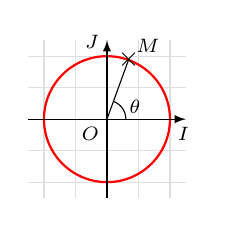
\begin{tikzpicture}[scale = 0.4]
        \draw[thin, color=gray!25] (-2.5,-2.5) grid (2.5,2.5);
        \draw[red,thick] (0,0) circle (2cm);
        \draw[->,>=latex] (-2.5,0)--(2.5,0);
        \draw[->,>=latex] (0,-2.5)--(0,2.5);
        \coordinate (O) at (0,0);
        \coordinate (I) at (2,0);
        \coordinate (J) at (0,2);
        \coordinate (M) at (70:2cm);
        \draw (M) node {$\times$};
        \begin{scriptsize}
            \draw (O) node[below left]{$O$};
            \draw (I) node[below right]{$I$};
            \draw (J) node[above left]{$J$};
            \draw (M) node [above right] {$M$};
            \draw (O) -- (M);
            \draw (0.6,0) arc (0:70:0.6cm);
            \draw (40:0.6cm) node[right] {$\theta$};
        \end{scriptsize}
    \end{tikzpicture}
    \end{center}
\end{Rmq}

\begin{Defi}
    Dans le cercle trigométrique, on appelle \ipt{sens trigonométrique}, ou sens direct, le sens qui parcourt le cercle dans le sens inverse des aiguilles d'une montre.\par
    Dans le sens trigonométrique, la mesure d'un angle sera positive ; dans le sens indirect, la mesure sera négative.
    \begin{center}
    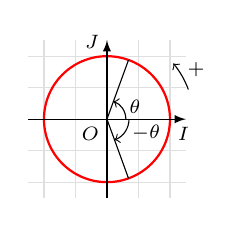
\begin{tikzpicture}[scale = 0.4]
        \draw[thin, color=gray!25] (-2.5,-2.5) grid (2.5,2.5);
        \draw[red,thick] (0,0) circle (2cm);
        \draw[->,>=latex] (-2.5,0)--(2.5,0);
        \draw[->,>=latex] (0,-2.5)--(0,2.5);
        \coordinate (O) at (0,0);
        \coordinate (I) at (2,0);
        \coordinate (J) at (0,2);
        \coordinate (M) at (70:2cm); \draw (O) -- (M);
        \coordinate (N) at (-70:2cm); \draw (O) -- (N);
        \draw[->] (20:2.75cm) arc (20:40:2.75cm);
        \draw (35:2.75cm) node[right] {\scriptsize $+$};
        \begin{scriptsize}
            \draw (O) node[below left]{$O$};
            \draw (I) node[below right]{$I$};
            \draw (J) node[above left]{$J$};
            \draw[->] (0.6,0) arc (0:70:0.6cm);
            \draw (40:0.6cm) node[right] {$\theta$};
            \draw[->] (0.7,0) arc (0:-70:0.7cm);
            \draw (-40:0.7cm) node[right] {$-\theta$};
        \end{scriptsize}
    \end{tikzpicture}
    \end{center}
\end{Defi}

\subsection{Mesurer un angle en radian}

\begin{Defi}
    On considère le cercle trigonométrique $\calig U$ ainsi qu'un point $M$ sur ce cercle.\par
    La mesure de l'angle $\widehat{IOM}$, exprimée en \ipt{radian}, est égale à la longueur de l'arc $\Arc{IM}$ dans le sens trigonométrique et est égale à l'opposé de la longueur de l'arc $\Arc{IM}$ dans le sens indirect.

\begin{center}
    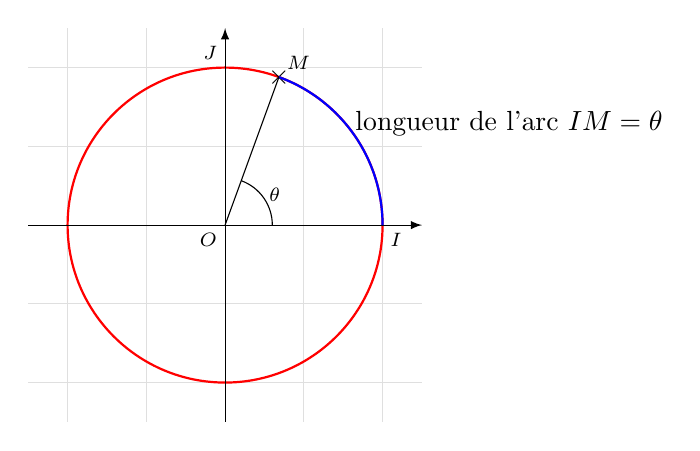
\begin{tikzpicture}
        \draw[thin, color=gray!25] (-2.5,-2.5) grid (2.5,2.5);
        \draw[red,thick] (0,0) circle (2cm);
        \draw[->,>=latex] (-2.5,0)--(2.5,0);
        \draw[->,>=latex] (0,-2.5)--(0,2.5);
        \coordinate (O) at (0,0);
        \coordinate (I) at (2,0);
        \coordinate (J) at (0,2);
        \coordinate (M) at (70:2cm);
        \draw (M) node {$\times$};
        \draw[thick,blue] (2,0) arc (0:70:2cm);
        \draw (40:2cm) node[right] {longueur de l'arc $\Arc{IM} = \theta$};
        \begin{scriptsize}
            \draw (O) node[below left]{$O$};
            \draw (I) node[below right]{$I$};
            \draw (J) node[above left]{$J$};
            \draw (M) node [above right] {$M$};
            \draw (O) -- (M);
            \draw (0.6,0) arc (0:70:0.6cm);
            \draw (40:0.6cm) node[right] {$\theta$};
        \end{scriptsize}
    \end{tikzpicture}
\end{center}
\end{Defi}

\begin{Exemple}[s]
\begin{enumerate}
    \item Lorsque le point $M$ est confondu au point $I$, la longueur de l'arc $\Arc{IM}$ est égal à $0$ donc on obtient $\widehat{IOM} = 0 \text{ rad}$.
    \item Si on suppose maintenant que le point $M$ a effectué un tour complet autour du cercle dans le sens trigonométrique, on trouve que la longueur de l'arc $\Arc{IM}$ est égal au périmètre $\calig P$ du cercle. Or, $\calig P = 2\pi r$ et $r = 1$ donc on obtient $\widehat{IOM} = 2\pi \text{ rad}$.
    \item Si on effectue à présent un quart de tour dans le sens direct, on aura $\widehat{IOM} = \frac{2\pi}{4} = \frac\pi2 \text{ rad}$.
    \item Si on effectue à présent un quart de tour dans le sens indirect, on aura $\widehat{IOM} = -\frac{2\pi}{4} = -\frac\pi2 \text{ rad}$.
\begin{center}
    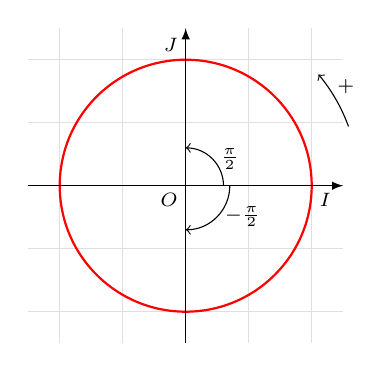
\begin{tikzpicture}[scale=0.8]
        \draw[thin, color=gray!25] (-2.5,-2.5) grid (2.5,2.5);
        \draw[red,thick] (0,0) circle (2cm);
        \draw[->,>=latex] (-2.5,0)--(2.5,0);
        \draw[->,>=latex] (0,-2.5)--(0,2.5);
        \coordinate (O) at (0,0);
        \coordinate (I) at (2,0);
        \coordinate (J) at (0,2);
        \coordinate (M) at (90:2cm); \draw (O) -- (M);
        \coordinate (N) at (-90:2cm); \draw (O) -- (N);
        \draw[->] (20:2.75cm) arc (20:40:2.75cm);
        \draw (35:2.75cm) node[right] {\scriptsize $+$};
        \begin{scriptsize}
            \draw (O) node[below left]{$O$};
            \draw (I) node[below right]{$I$};
            \draw (J) node[above left]{$J$};
            \draw[->] (0.6,0) arc (0:90:0.6cm);
            \draw (45:0.6cm) node[right] {$\frac\pi 2$};
            \draw[->] (0.7,0) arc (0:-90:0.7cm);
            \draw (-45:0.7cm) node[right] {$-\frac\pi 2$};
        \end{scriptsize}
    \end{tikzpicture}
    \end{center}
\end{enumerate}
\end{Exemple}\medskip

L'exemple précédent nous montre qu'une même position pour le point $M$ peut entraîner différentes mesures d'un angle, en fonction du nombre de tours effectués par $M$. Les différentes mesures diffèrent donc d'un multiple de $2\pi$ qui correspond au périmètre du cercle trigonométrique. On a donc :

\begin{Prop}
    On considère un point $M$ sur le cercle $\calig U$.
    \begin{enumerate}
        \item L'angle $\widehat{IOM}$ possède une infinité de mesure.
        \item Pour deux mesures $x$ et $y$, il existe $k \in \Z$ tel que $y = x + 2k\pi$.
        \item Il n'existe qu'une seule mesure dans l'intervalle $\intervalleof{-\pi}{\pi}$.
    \end{enumerate}
\end{Prop} \medskip

Afin de garantir l'unicité de certains résultats, on est amené à définir la notion de mesure principale d'un angle :

\begin{Defi}
    On considère un point $M$ sur le cercle $\calig U$.
    Parmi toutes les mesures de l'angle $\widehat{IOM}$, on appelle \ipt{mesure principale} celle qui appartient à l'intervalle $\intervalleof{-\pi}{\pi}$.
\end{Defi}\clearpage

\begin{Exemple}
    On considère un angle de mesure $\alpha = \frac{43\pi}{4}$. Déterminer la mesure principale de cet angle et placer $M$ sur $\calig U$ tel que $\widehat{IOM} = \alpha$.\par\medskip
    Il suffit de trouver $k \in \Z$ tel que $\frac{43\pi}{4} = x + 2k\pi$ et $x$ sera alors la mesure principale cherchée.\par
    On réduit tout d'abord au même dénominateur : $2\pi = \frac{8\pi}{4}$ puis on effectue la division euclidienne de $43$ par $8$ : $43 =5\times 8 + 3$.\par\medskip
    Ainsi : $\frac{43\pi}{4} = \frac{5 \times 8\pi}{4} + \frac{3\pi}{4} = 5 \times 2\pi + \frac{3\pi}{4}$ donc la mesure principale de l'angle est $\frac{3\pi}{4}$.

\begin{center}
    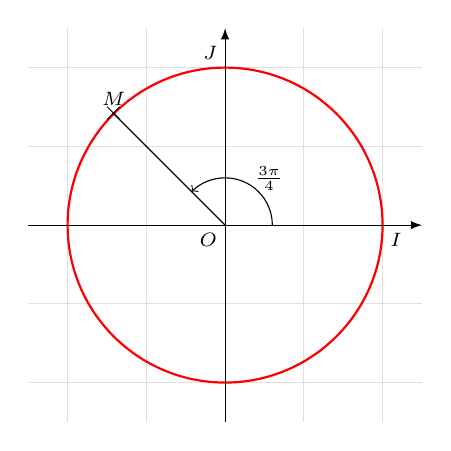
\begin{tikzpicture}
        \draw[thin, color=gray!25] (-2.5,-2.5) grid (2.5,2.5);
        \draw[red,thick] (0,0) circle (2cm);
        \draw[->,>=latex] (-2.5,0)--(2.5,0);
        \draw[->,>=latex] (0,-2.5)--(0,2.5);
        \coordinate (O) at (0,0);
        \coordinate (I) at (2,0);
        \coordinate (J) at (0,2);
        \coordinate (M) at (135:2cm);
        \draw (M) node {$\times$};
        \begin{scriptsize}
            \draw (O) node[below left]{$O$};
            \draw (I) node[below right]{$I$};
            \draw (J) node[above left]{$J$};
            \draw (M) node [above] {$M$};
            \draw (O) -- (M);
            \draw[->] (0.6,0) arc (0:135:0.6cm);
            \draw (80:0.6cm) node[right=5pt] {$\frac{3\pi}{4}$};
        \end{scriptsize}
    \end{tikzpicture}
    \end{center}
\end{Exemple}

\subsection{Quelques conversions à connaître}

\begin{center}
\renewcommand\arraystretch{2.5}
    \begin{tabular}{*{10}{|c}|}
        \hline
            Angles en degré & $0$ & $360$ & $180$ & $30$ & $45$ & $60$ & $90$ & $270$ & $\alpha$ \\
        \hline
            Angles en radian & $0$ & $2\pi$ & $\frac\pi2$ & $\frac{\pi}{6}$ & $\frac\pi4$ & $\frac\pi3$ & $\frac\pi2$ & $\frac{3\pi}{2}$  & $\alpha \times\frac{2\pi}{360}$\\
        \hline
    \end{tabular}
\end{center}

\section{Cosinus et Sinus d'un nombre réel}
\subsection{Lien avec le cercle trigonométrique}

\begin{Prop}
    On considère un point $M$ sur le cercle $\calig U$ et $\alpha$ un nombre réel tel que $\widehat{IOM} = \alpha$. On ne demande pas à $\alpha$ d'être la mesure principale de l'angle $\widehat{IOM}$.\par
    Le nombre \iptb{$\cos(\alpha)$}\index{cosinus d'un nombre réel} est alors égal à l'abscisse du point $M$ et le nombre \iptb{$\sin(\alpha)$}\index{sinus d'un nombre réel} est égal à l'ordonnée du point $M$.

\begin{center}
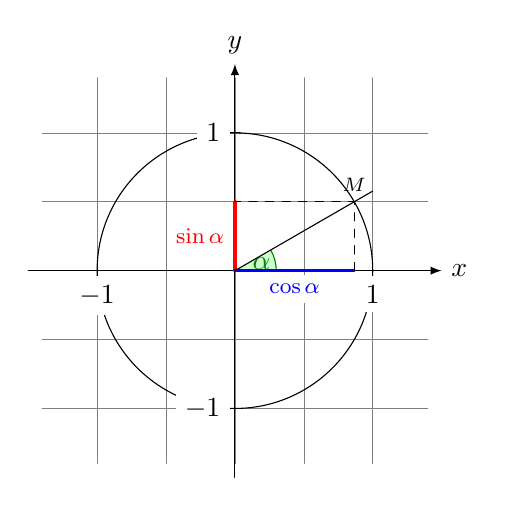
\begin{tikzpicture}[scale=1.75,cap=round]
    % Local definitions
    \def\costhirty{0.8660256}
    % Colors
    \colorlet{anglecolor}{green!50!black}
    \colorlet{sincolor}{red}
    \colorlet{tancolor}{orange!80!black}
    \colorlet{coscolor}{blue}
    % Styles
    \tikzstyle{axes}=[>=latex]
    \tikzstyle{important line}=[very thick]
    \tikzstyle{information text}=[rounded corners,fill=red!10,inner sep=1ex]
    % The graphic
    \draw[style=help lines,step=0.5cm] (-1.4,-1.4) grid (1.4,1.4);
    \draw (0,0) circle (1cm);
    \begin{scope}[style=axes]
        \draw[->] (-1.5,0) -- (1.5,0) node[right] {$x$} coordinate(x axis);
        \draw[->] (0,-1.5) -- (0,1.5) node[above] {$y$} coordinate(y axis);
        \foreach \x in {-1,1} \draw[xshift=\x cm] (0pt,1pt) -- (0pt,-1pt) node[below,fill=white] {$\x$};
        \foreach \y in {-1,1} \draw[yshift=\y cm] (1pt,0pt) -- (-1pt,0pt) node[left,fill=white] {$\y$};
    \end{scope}
    \filldraw[fill=green!20,draw=anglecolor] (0,0) -- (3mm,0pt) arc(0:30:3mm);
    \draw (15:2mm) node[anglecolor] {$\alpha$};
    \draw[style=important line,sincolor] (0,0) -- node[left,fill=white] {\footnotesize$\sin \alpha$} (0,0.5);
    \draw[style=important line,coscolor] (30:1cm |- x axis) -- node[below=1pt,fill=white] {\footnotesize$\cos \alpha$} (0,0);
    \draw[dashed] (30:1cm |- x axis) -- (30:1cm) -- (30:1cm -| y axis);
    \draw (intersection of 0,0--30:1cm and 1,0--1,1) coordinate (t);
    \draw (0,0) -- (t);
    \draw (30:1cm) node[above] {\scriptsize$M$};
\end{tikzpicture}
\end{center}
\end{Prop}\clearpage

\begin{Demo}
L'unité de longueur étant fixée, on utilise les définitions données du cosinus et du sinus d'un angle aigu $\alpha$ dans le triangle rectangle :
\[\cos(\alpha) = \frac{\text{côté adjacent}}{\text{hypoténuse}} \qetq \sin(\alpha) = \frac{\text{côté opposé}}{\text{hypoténuse}}\]
On considère dans la figure ci-dessous les triangles $OMH$ et $OMK$ rectangles respectivement en $H$ et en $K$.\par
Les angles $\widehat{HOM}$ et $\widehat{KMO}$ sont alternes-internes. Et comme les droites ($OH)$ et $(MK)$ sont parallèles alors les angles $\widehat{HOM}$ et $\widehat{KMO}$ sont égaux donc $\widehat{KMO} = \alpha$.

\begin{center}
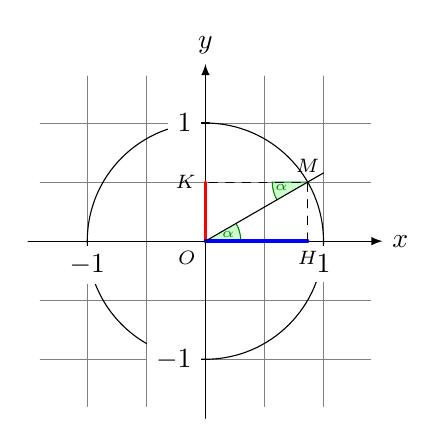
\begin{tikzpicture}[scale=1.5,cap=round]
    % Local definitions
    \def\costhirty{0.8660256}
    % Colors
    \colorlet{anglecolor}{green!50!black}
    \colorlet{sincolor}{red}
    \colorlet{tancolor}{orange!80!black}
    \colorlet{coscolor}{blue}
    % Styles
    \tikzstyle{axes}=[>=latex]
    \tikzstyle{important line}=[very thick]
    \tikzstyle{information text}=[rounded corners,fill=red!10,inner sep=1ex]
    % The graphic
    \draw[style=help lines,step=0.5cm] (-1.4,-1.4) grid (1.4,1.4);
    \draw (0,0) circle (1cm);
    \begin{scope}[style=axes]
        \draw[->] (-1.5,0) -- (1.5,0) node[right] {$x$} coordinate(x axis);
        \draw[->] (0,-1.5) -- (0,1.5) node[above] {$y$} coordinate(y axis);
        \foreach \x in {-1,1} \draw[xshift=\x cm] (0pt,1pt) -- (0pt,-1pt) node[below,fill=white] {$\x$};
        \foreach \y in {-1,1} \draw[yshift=\y cm] (1pt,0pt) -- (-1pt,0pt) node[left,fill=white] {$\y$};
    \end{scope}
    \filldraw[fill=green!20,draw=anglecolor] (0,0) -- (3mm,0pt) arc(0:30:3mm);
    \draw (15:2mm) node[anglecolor] {\tiny$\alpha$};
    \filldraw[fill=green!20,draw=anglecolor] (\costhirty,0.5) -- ++(-3mm,0pt) arc(180:210:3mm);
    \draw (30:0.9cm) node[anglecolor,left] {\tiny$\alpha$};
    \draw[style=important line,sincolor] (0,0) -- (0,0.5);
    \draw[style=important line,coscolor] (30:1cm |- x axis) -- (0,0);
    \draw[dashed] (30:1cm |- x axis) -- (30:1cm) -- (30:1cm -| y axis);
    \draw (intersection of 0,0--30:1cm and 1,0--1,1) coordinate (t);
    \draw (0,0) -- (t);
    \draw (30:1cm) node[above] {\scriptsize$M$};
    \draw (\costhirty,0) node[below] {\scriptsize$H$};
    \draw (0,0.5) node[left] {\scriptsize$K$};
    \draw (0,0) node[below left] {\scriptsize$O$};
\end{tikzpicture}
\end{center}

Les triangles $OKM$ et $OHM$ ont la même hypoténuse $[OM]$ qui est un rayon du cercle. Donc $OM = 1$.
On utilise les définitions et on a :
\[\cos(\alpha) = \frac{OH}{OM} = OH \qetq \sin(\alpha) = \frac{OK}{OM} = OH.\]
\end{Demo}

\subsection{Relations à connaître}

\begin{Prop}
    On considère un angle de mesure $\theta$. On a les relations suivantes :
    \begin{enumerate}
        \item $\cos(-\theta) = \cos(\theta)$ et $\sin(-\theta) = -\sin(\theta)$.
        \item $\cos(\pi -\theta) = -\cos(\theta)$ et $\sin(\pi-\theta) = \sin(\theta)$.
    \end{enumerate}
\end{Prop}

\begin{Demo}
    Le plus simple est d'utiliser une figure géométrique :

    \begin{center}
        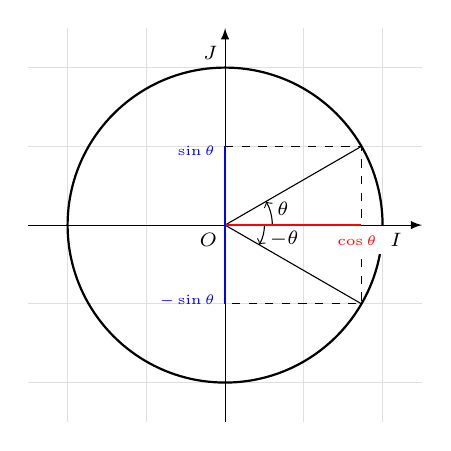
\begin{tikzpicture}
            \draw[thin, color=gray!25] (-2.5,-2.5) grid (2.5,2.5);
            \draw[thick] (0,0) circle (2cm);
            \draw[->,>=latex] (-2.5,0)--(2.5,0);
            \draw[->,>=latex] (0,-2.5)--(0,2.5);
            \coordinate (O) at (0,0);
            \coordinate (I) at (2,0);
            \coordinate (J) at (0,2);
            \coordinate (M) at (30:2cm); \draw (O) -- (M);
            \coordinate (N) at (-30:2cm); \draw (O) -- (N);
            \begin{scriptsize}
                \draw (O) node[below left]{$O$};
                \draw (I) node[below right]{$I$};
                \draw (J) node[above left]{$J$};
                \draw[->] (0.6,0) arc (0:30:0.6cm);
                \draw (20:0.6cm) node[right] {$\theta$};
                \draw[->] (0.5,0) arc (0:-30:0.5cm);
                \draw (-20:0.5cm) node[right] {$-\theta$};
            \end{scriptsize}
            \draw[dashed] (0,1) --({2*0.8660256},1) -- ({2*0.8660256},-1) -- (0,-1);
            \draw[red,thick] (0,0) -- ({2*0.8660256},0) node[below right, near end,fill=white]{\tiny $\cos\theta$};
            \draw[blue,thick] (0,0) -- (0,1) node[above left, near end]{\tiny $\sin\theta$};
            \draw[blue,thick] (0,0) -- (0,-1) node[below left, near end]{\tiny $-\sin\theta$};
        \end{tikzpicture}
        \hspace{1cm}
        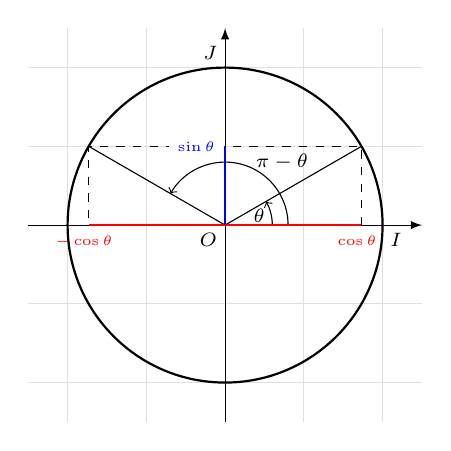
\begin{tikzpicture}
            \draw[thin, color=gray!25] (-2.5,-2.5) grid (2.5,2.5);
            \draw[thick] (0,0) circle (2cm);
            \draw[->,>=latex] (-2.5,0)--(2.5,0);
            \draw[->,>=latex] (0,-2.5)--(0,2.5);
            \coordinate (O) at (0,0);
            \coordinate (I) at (2,0);
            \coordinate (J) at (0,2);
            \coordinate (M) at (30:2cm); \draw (O) -- (M);
            \coordinate (N) at (150:2cm); \draw (O) -- (N);
            \begin{scriptsize}
                \draw (O) node[below left]{$O$};
                \draw (I) node[below right]{$I$};
                \draw (J) node[above left]{$J$};
                \draw[->] (0.6,0) arc (0:30:0.6cm);
                \draw (15:0.45cm) node {$\theta$};
                \draw[->] (0.8,0) arc (0:150:0.8cm);
                \draw (70:0.85cm) node[right] {$\pi-\theta$};
            \end{scriptsize}
            \draw[dashed] ({2*0.8660256},0) -- ({2*0.8660256},1) -- ({-2*0.8660256},1) -- ({-2*0.8660256},0);
            \draw[red,thick] (0,0) -- ({2*0.8660256},0) node[below right, near end]{\tiny $\cos\theta$};
            \draw[red,thick] (0,0) -- ({-2*0.8660256},0) node[below left, near end]{\tiny $-\cos\theta$};
            \draw[blue,thick] (0,0) -- (0,1) node[fill=white,left]{\tiny $\sin\theta$};
        \end{tikzpicture}
    \end{center}
\end{Demo}

\subsection{Quelques équations trigonométriques}
La propriété précédente nous permet alors de résoudre quelques équations où apparaissent soit le cosinus, soit le sinus.

\begin{Prop}
    Soit $a$ un nombre fixé.\par
    L'équation $\cos (t) = \cos (a)$ admet une \textbf{infinité} de solutions pouvant s'écrire sous l'une des deux formes suivantes :
    \[t = a + 2k\pi, k \in \Z \qquad \text{ou} \qquad t = -a + 2k\pi, k \in \Z\]
\end{Prop}

\begin{Exemple}
    Donner toutes les solutions de l'équation suivantes puis la mesure principale des angles qui vérifient l'équation :
    \[\cos(t) = \cos\left(\frac\pi3\right).\]
    Les solutions sont de la forme $t = \frac\pi3 + 2k\pi (k \in Z)$ ou $t = -\frac\pi3 + 2k\pi (k \in \Z)$.\par
    Par exemple, voici quelques solutions :
    \[
    \renewcommand\arraystretch{2.75}
    \begin{array}{|c|c|c|}
    \hline
        k = 0 & \frac\pi3 & -\frac\pi3\\
    \hline
        k = 1 & \frac{7\pi}{3} & \frac{5\pi}{3}\\
    \hline
        k = -1 & -\frac{5\pi}{3} & -\frac{7\pi}{3}\\
    \hline
        k = 2 & \frac{13\pi}{3} & \frac{11\pi}{3} \\
    \hline
        k = -2 & -\frac{11\pi}{3} & -\frac{13\pi}{3} \\
    \hline
    \end{array}
    \]
    $\frac \pi 3$ et $-\frac\pi3$ sont les mesures principales des angles solutions.
\end{Exemple}

\begin{Prop}
    Soit $a$ un nombre fixé.\par
    L'équation $\sin (t) = \sin (a)$ admet une \textbf{infinité} de solutions pouvant s'écrire sous l'une des deux formes suivantes :
    \[t = a + 2k\pi, k \in \Z \qquad \text{ou} \qquad t = \pi -a + 2k\pi, k \in \Z\]
\end{Prop}

\begin{Exemple}
    Donner toutes les solutions de l'équation suivantes puis la mesure principale des angles qui vérifient l'équation :
    \[\sin(t) = \sin\left(\frac\pi6\right).\]
    Les solutions sont de la forme $t = \frac\pi6 + 2k\pi (k \in Z)$ ou $t = \underbrace{\pi-\frac\pi6}_{=\frac{5\pi}{6}} + 2k\pi (k \in \Z)$.\par
    Par exemple, voici quelques solutions :
    \[
    \renewcommand\arraystretch{2.75}
    \begin{array}{|c|c|c|}
    \hline
        k = 0 & k = 1 & k = -1\\
    \hline
        \frac\pi6 & \frac{13\pi}{6} & -\frac{11\pi}{6}\\
    \hline
        \frac{5\pi}{6} & \frac{17\pi}{6} & -\frac{7\pi}{6}\\
    \hline
    \end{array}
    \]
    $\frac \pi 6$ et $\frac{5\pi}{6}$ sont les mesures principales des angles solutions.
\end{Exemple}

\end{document}


%------ Index
\setcounter{tocdepth}{1}
    %------ Index
\renewenvironment{theindex}
{\cleardoublepage
{\color{\MaCouleur}
       \vspace*{10\p@}%
        \begin{minipage}[c]{\textwidth}
        \rule{\textwidth}{1ex}
        \par\nobreak
        \begin{flushright}
            \Huge\bfseries Index \\ des notions définies
         \end{flushright}
        \par\nobreak
        \rule{\textwidth}{1ex}
         \end{minipage}
    \vskip 40\p@
}
\renewcommand{\item}{\par\hangindent 40pt}
\begin{multicols}{2}
}
{\end{multicols}}

\entete{}{}{}
\printindex\addcontentsline{toc}{chapter}{\protect Index des notions définies}

\vspace{\stretch{1}}

\[***\]

\begin{center}
\'Ecrit par Philippe \bsc{De Sousa}.\par
Dernière modification le \today.
\end{center}

\end{document} 